%
% Stony Brook University Spring 2013 Senior Thesis
%
% Ryan Orvedahl Spring 2013

%\documentclass[titlepage,12pt]{article}
%\documentclass[apj]{emulateapj}
%\documentclass[apj,onecolumn]{emulateapj}
\documentclass[apj,twocolumn]{emulateapj} 
%\bibliographystyle{apj}

% Define new commands (shortcuts):
\input shortcuts

% allows the \hl{} command to highlight stuff
\usepackage{color,soul}

%\usepackage{pdflscape} % landscape ability
%\usepackage{scrextend} % footnote and \footref commands

\begin{document}

%========================================================================
% create title and author
%========================================================================
\title{Simulations of the Tayler-Spruit Dynamo}
\author{Ryan J. Orvedahl$^{1,2}$, Benjamin P. Brown$^{1,3}$, 
        Juri Toomre$^{1,2}$}
\affil{$^1$Department of Astrophysical \& Planetary Scienes, University of 
       Colorado, Boulder, CO 80309-0391, USA}
\affil{$^2$JILA, University of Colorado, Boulder, CO 80309-0440, USA}
\affil{$^3$Laboratory for Atmospheric and Space Physics, University of 
       Colorado, Boulder, CO 80303-7814, USA}

%\date{\today}

%%%%%%%%%%%%%%%%%%%%%%%%%%%%%%%%%%%%%%%%%%%%%%%%%%%%%%%%%%%%%%%%%%%%%%%%
% Abstract
%%%%%%%%%%%%%%%%%%%%%%%%%%%%%%%%%%%%%%%%%%%%%%%%%%%%%%%%%%%%%%%%%%%%%%%%
\begin{abstract}
Many phenomena in Astrophysics are largely subsonic and require special
\end{abstract}

\keywords{Magnetohydrodynamics, Computational Fluid Dynamics, Dynamo}

\maketitle


%%%%%%%%%%%%%%%%%%%%%%%%%%%%%%%%%%%%%%%%%%%%%%%%%%%%%%%%%%%%%%%%%%%%%%%%
% Intro
%%%%%%%%%%%%%%%%%%%%%%%%%%%%%%%%%%%%%%%%%%%%%%%%%%%%%%%%%%%%%%%%%%%%%%%%
\input intro


%%%%%%%%%%%%%%%%%%%%%%%%%%%%%%%%%%%%%%%%%%%%%%%%%%%%%%%%%%%%%%%%%%%%%%%%
% Problem Setup
%%%%%%%%%%%%%%%%%%%%%%%%%%%%%%%%%%%%%%%%%%%%%%%%%%%%%%%%%%%%%%%%%%%%%%%%
\section{Problem Setup}
\label{sec:flame}
To model astrophysical thermonuclear flames using \maestro, a cool fuel and 


%%%%%%%%%%%%%%%%%%%%%%%%%%%%%%%%%%%%%%%%%%%%%%%%%%%%%%%%%%%%%%%%%%%%%%%%
% Results
%%%%%%%%%%%%%%%%%%%%%%%%%%%%%%%%%%%%%%%%%%%%%%%%%%%%%%%%%%%%%%%%%%%%%%%%
\section{Results}
\label{sec:results}
Using the \maestro\ code, I ran many different flame experiments. I varied 


%%%%%%%%%%%%%%%%%%%%%%%%%%%%%%%%%%%%%%%%%%%%%%%%%%%%%%%%%%%%%%%%%%%%%%%%
% Conclusions
%%%%%%%%%%%%%%%%%%%%%%%%%%%%%%%%%%%%%%%%%%%%%%%%%%%%%%%%%%%%%%%%%%%%%%%%
\section{Conclusions and Discussion}
\label{sec:conclusions}
Studying the dynamics of flames in low Mach number environments is a difficult 


%%%%%%%%%%%%%%%%%%%%%%%%%%%%%%%%%%%%%%%%%%%%%%%%%%%%%%%%%%%%%%%%%%%%%%%%
% Acknowledgements
%%%%%%%%%%%%%%%%%%%%%%%%%%%%%%%%%%%%%%%%%%%%%%%%%%%%%%%%%%%%%%%%%%%%%%%%
%\section*{\hl{Acknowledgements}}
%\label{sec:acks}

\bigskip
We thank Ellen (\hl{include as author?}), SPIDER for their suggestions and 
advice. This research is partly supported by NASA \hl{...?} Orvedahl is 
supported through \hl{a Hale Fellowship}. Brown is supported through \hl{...}. 
Toomre is supported through \hl{...}. The simulations were carried out with 
\hl{Janus supported by ...} and with NASA HECC support of Pleiades.


%%%%%%%%%%%%%%%%%%%%%%%%%%%%%%%%%%%%%%%%%%%%%%%%%%%%%%%%%%%%%%%%%%%%%%%%
% Appendix
%%%%%%%%%%%%%%%%%%%%%%%%%%%%%%%%%%%%%%%%%%%%%%%%%%%%%%%%%%%%%%%%%%%%%%%%
\input appendix


%%%%%%%%%%%%%%%%%%%%%%%%%%%%%%%%%%%%%%%%%%%%%%%%%%%%%%%%%%%%%%%%%%%%%%%%
% References
%%%%%%%%%%%%%%%%%%%%%%%%%%%%%%%%%%%%%%%%%%%%%%%%%%%%%%%%%%%%%%%%%%%%%%%%
% include references
%\nocite{*}
\bibliography{Bibliography}


%%%%%%%%%%%%%%%%%%%%%%%%%%%%%%%%%%%%%%%%%%%%%%%%%%%%%%%%%%%%%%%%%%%%%%%%
% Figures
%%%%%%%%%%%%%%%%%%%%%%%%%%%%%%%%%%%%%%%%%%%%%%%%%%%%%%%%%%%%%%%%%%%%%%%%

%======================================================================
% the figure* environment allows the figure to take up two columns
%\begin{figure*}[h]
%\begin{center}
%\centerline{\includegraphics[scale=0.4,angle=0]{./Plots/.pdf}}
%\caption{}
%\label{fig:}
%\end{center}
%\end{figure*}

%======================================================================
\begin{figure*}[h]
\begin{center}
\centerline{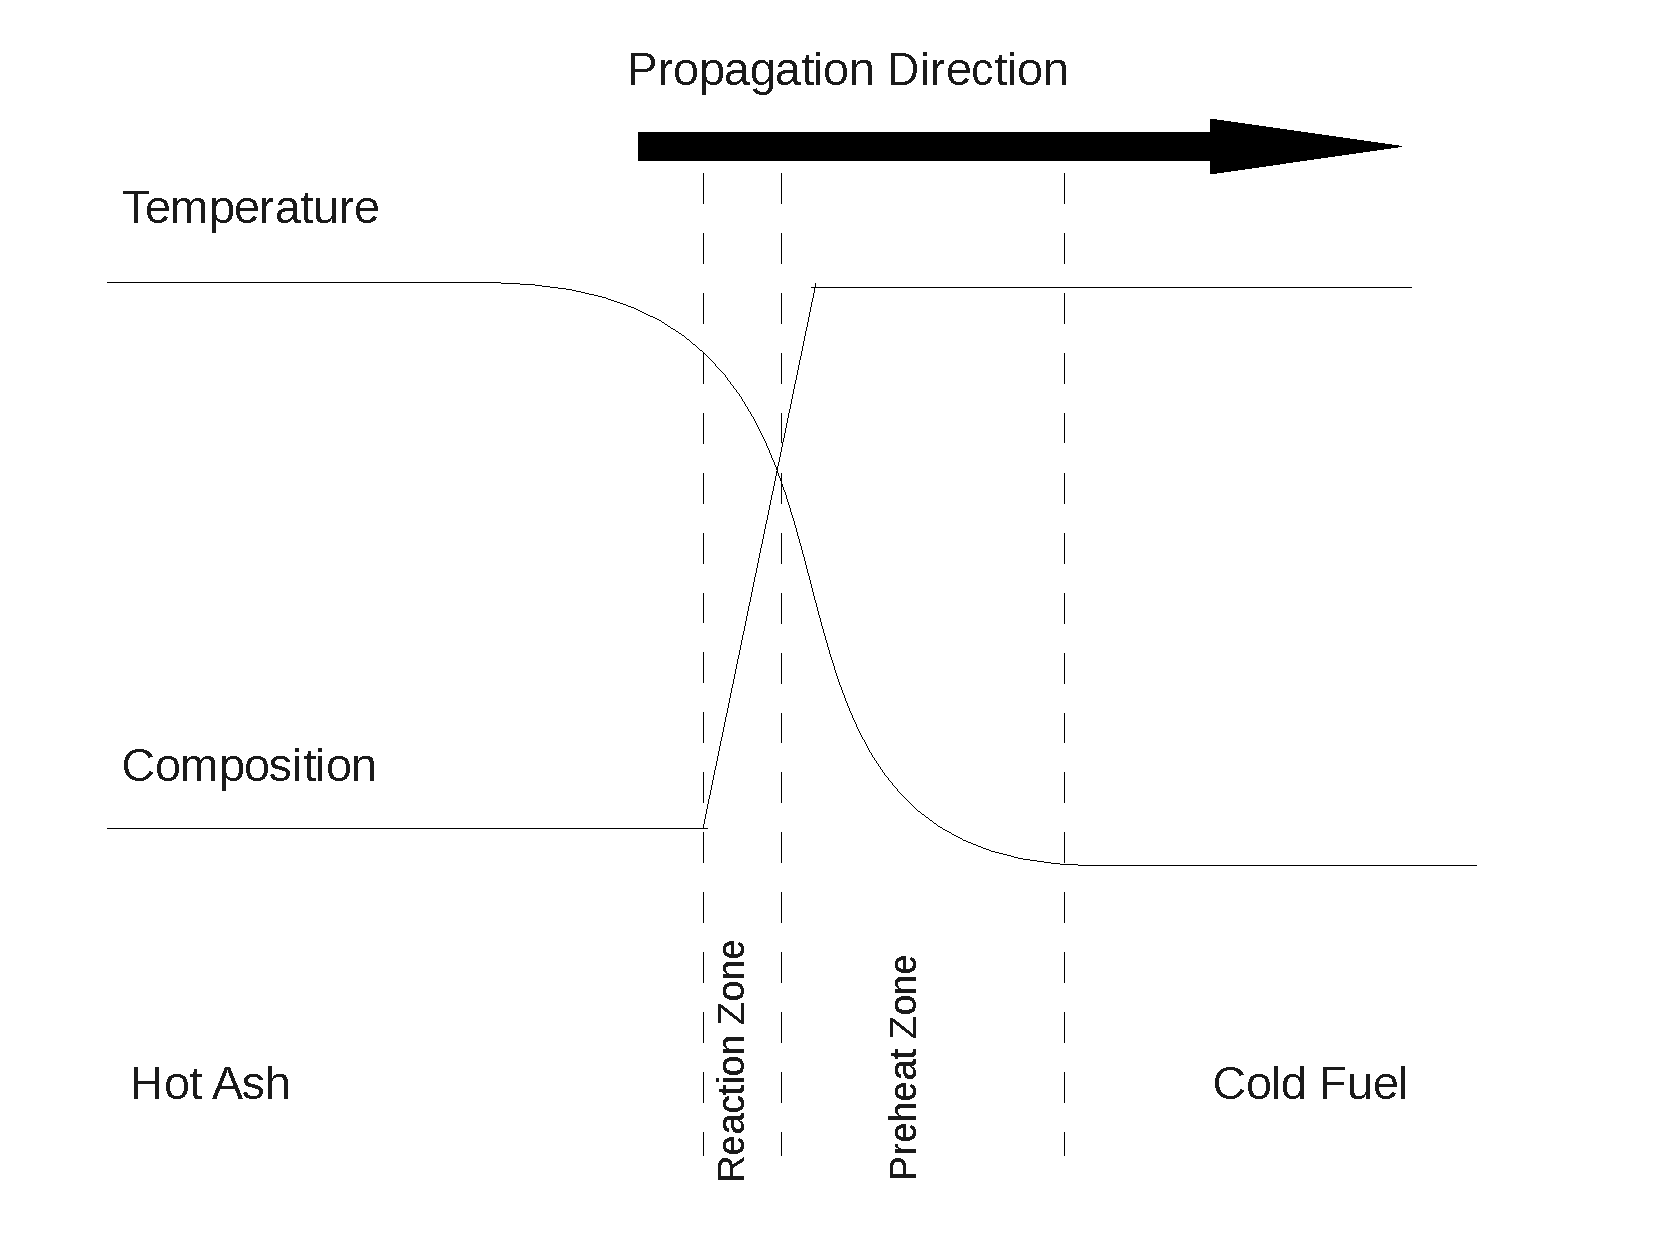
\includegraphics[scale=0.4,angle=0]{./Plots/flame_schematic.pdf}}
\caption{Schematic of an astrophysical flame propagating to the right. The 
reactions are strongly peaked in the thin reaction zone \citep{flamecurve}.}
\label{fig:flame}
\end{center}
\end{figure*}

%======================================================================
% Density = 10^7, CFL = 0.5, VARY THE RESOLUTION
%  \begin{figure*}[!htb]
%    \minipage{0.30\textwidth}
%       \includegraphics[scale=0.3,angle=0]{./Plots/simple_cfl5_dens7_res5_nosdc.pdf}
%       \caption{Simple-3, Resolution = 5, $\rho = 10^7$, CFL = 0.5, Non-SDC}
%       \label{fig:lowres}
%    \endminipage
%    \hfill
%    \minipage{0.30\textwidth}
%       \includegraphics[scale=0.3,angle=0]{./Plots/simple_cfl5_dens7_res10_nosdc.pdf}
%       \caption{Simple-3, Resolution = 10, $\rho = 10^7$, CFL = 0.5, Non-SDC}
%       \label{fig:medres}
%    \endminipage
%    \hfill
%    \minipage{0.30\textwidth}
%       \includegraphics[scale=0.3,angle=0]{./Plots/simple_cfl5_dens7_res20_nosdc.pdf}
%       \caption{Simple-3, Resolution = 20, $\rho = 10^7$, CFL = 0.5, Non-SDC}
%       \label{fig:highres}
%    \endminipage
%  \end{figure*}


%%%%%%%%%%%%%%%%%%%%%%%%%%%%%%%%%%%%%%%%%%%%%%%%%%%%%%%%%%%%%%%%%%%%%%%%
% Data
%%%%%%%%%%%%%%%%%%%%%%%%%%%%%%%%%%%%%%%%%%%%%%%%%%%%%%%%%%%%%%%%%%%%%%%%

%======================================================================
\begin{table}[h]
\begin{center}
\begin{tabular}{|c|c|c|c|}
\hline
& Simple-3 (\maestro) & Regular-9 (\mesa)& Extended-33 (\mesa) \\ \hline
1 & C12 & H1 & neutron \\ \hline
2 & O16 & He4 & H1 \\ \hline
3 & Mg24 & C12 & He3 \\ \hline
4 & - & O16 & He4\\ \hline
5 & - & Ne20 & Be9\\ \hline
6 & - & Na23 & C12\\ \hline
7 & - & Mg23 & C13\\ \hline
8 & - & Mg24 & N13\\ \hline
9 & - & Si28 & N14\\ \hline
10 & - & - & N15\\ \hline
11 & - & - & O15\\ \hline
12 & - & - & ...\\ \hline
\end{tabular}
\caption{List of isotopes used in each network. The Regular-9 and Extended-33 
networks used the \mesa\ code while the Simple-3 network used the \maestro\ 
code.}
\label{tab:isos}
\end{center}
\end{table}

\end{document}


